%%%%%%%%%%%%%%%%%%%%%%%%%%%%%%%%%%%%%%%%%
% Beamer Presentation
% LaTeX Template
% Version 1.0 (10/11/12)
%
% This template has been downloaded from:
% http://www.LaTeXTemplates.com
%
% License:
% CC BY-NC-SA 3.0 (http://creativecommons.org/licenses/by-nc-sa/3.0/)
%
%%%%%%%%%%%%%%%%%%%%%%%%%%%%%%%%%%%%%%%%%

%----------------------------------------------------------------------------------------
%	PACKAGES AND THEMES
%----------------------------------------------------------------------------------------

\documentclass[aspectratio=169]{beamer}
\usepackage{listings}

\usepackage{color}
\usepackage{xcolor}
\usepackage{booktabs}
\usepackage{enumitem}

\definecolor{mygray}{rgb}{0.4,0.4,0.4}
\definecolor{myorange}{rgb}{1.0,0.4,0}
\newcommand{\gr}{\cellcolor{green!40}}

\lstset{
basicstyle=\tiny\sffamily\color{black},
commentstyle=\color{mygray},
frame=single,
keywordstyle=\color{blue},
showspaces=false,
showstringspaces=false,
stringstyle=\color{myorange},
tabsize=2,
language=C++
}


\mode<presentation> {

% The Beamer class comes with a number of default slide themes
% which change the colors and layouts of slides. Below this is a list
% of all the themes, uncomment each in turn to see what they look like.

%\usetheme{default}
%\usetheme{AnnArbor}
%\usetheme{Antibes}
%\usetheme{Bergen}
%\usetheme{Berkeley}
%\usetheme{Berlin}
%\usetheme{Boadilla}
\usetheme{CambridgeUS}
%\usetheme{Copenhagen}
%\usetheme{Darmstadt}
%\usetheme{Dresden}
%\usetheme{Frankfurt}
%\usetheme{Goettingen}
%\usetheme{Hannover}
%\usetheme{Ilmenau}
%\usetheme{JuanLesPins}
%\usetheme{Luebeck}
%\usetheme{Madrid}
%\usetheme{Malmoe}
%\usetheme{Marburg}
%\usetheme{Montpellier}
%\usetheme{PaloAlto}
%\usetheme{Pittsburgh}
%\usetheme{Rochester}
%\usetheme{Singapore}
%\usetheme{Szeged}
%\usetheme{Warsaw}

% As well as themes, the Beamer class has a number of color themes
% for any slide theme. Uncomment each of these in turn to see how it
% changes the colors of your current slide theme.

%\usecolortheme{albatross}
%\usecolortheme{beaver}
%\usecolortheme{beetle}
%\usecolortheme{crane}
%\usecolortheme{dolphin}
%\usecolortheme{dove}
%\usecolortheme{fly}
%\usecolortheme{lily}
%\usecolortheme{orchid}
%\usecolortheme{rose}
%\usecolortheme{seagull}
%\usecolortheme{seahorse}
%\usecolortheme{whale}
%\usecolortheme{wolverine}

%\setbeamertemplate{footline} % To remove the footer line in all slides uncomment this line
%\setbeamertemplate{footline}[page number] % To replace the footer line in all slides with a simple slide count uncomment this line

\setbeamertemplate{navigation symbols}{} % To remove the navigation symbols from the bottom of all slides uncomment this line
}
\setbeamercovered{transparent}
\setbeamersize{text margin left=30pt,text margin right=30pt} 


\usepackage[utf8]{inputenc}
\usepackage{graphicx} % Allows including images
\usepackage{booktabs} % Allows the use of \toprule, \midrule and \bottomrule in tables

\setitemize{label=\usebeamerfont*{itemize item}%
  \usebeamercolor[fg]{itemize item}
  \usebeamertemplate{itemize item}}

\setlist[description]{leftmargin=\parindent, labelindent=\parindent}

%----------------------------------------------------------------------------------------
%	TITLE PAGE
%----------------------------------------------------------------------------------------

\title[Randomness Testing Toolkit]{The automated testing of randomness with multiple statistical batteries} % The short title appears at the bottom of every slide, the full title is only on the title page

\author[lubomir.obratil@gmail.com]{Ľubomír Obrátil\\lubomir.obratil@gmail.com} % Your name
\date{22. 6. 2017} % Date, can be changed to a custom date

% Eliminates margins
\def\nomar{\list{}{\rightmargin-30pt \leftmargin-30pt}\item[]}
\let\endnomar=\endlist

\usepackage{makecell}
\usepackage{xcolor, colortbl}

\renewcommand\theadfont{\bfseries}

\begin{document}

\begin{frame}
\titlepage % Print the title page as the first slide
\end{frame}

%----------------------------------------------------------------------------------------
%	PRESENTATION SLIDES
%----------------------------------------------------------------------------------------

%%%%%%%%%%%%%%%%%%%%%%%%%%%%%%%%%%%%
% Overview of the thesis structure %
%%%%%%%%%%%%%%%%%%%%%%%%%%%%%%%%%%%%
\begin{frame}
\frametitle{Thesis structure}

\begin{itemize}
\item Creation of a unified interface supporting multiple statistical batteries.
\begin{itemize}
\item NIST Statistical Testing Suite
\item Dieharder
\item TestU01
\end{itemize}
\item Conducting the baseline (control) experiment to create a reference point for the further experiments.
\item Evaluating randomness of outputs of well-known cryptographic primitives.
\item Analysing validity of the Dieharder battery results.
\end{itemize}

\end{frame}

%%%%%%%%%%%%%%%%%%%%%%%%%%%%%%%%%%%%%%%
% Randomness Testing Toolkit overview %
%%%%%%%%%%%%%%%%%%%%%%%%%%%%%%%%%%%%%%%
\begin{frame}
\frametitle{Randomness Testing Toolkit -- overview}
\begin{itemize}
\item Design and implementation of a tool for consistent randomness evaluation.
\item Intended to be used by users without prior knowledge about statistical testing as well as by researchers in CRoCS. 
\item The developed tool (RTT) acts as a interface between the user and the statistical batteries -- common format of the battery settings and results.
\item The toolkit supports multiple statistical batteries -- NIST STS, Dieharder and TestU01; it is possible to add more batteries over time.
\item Both standalone program and online service were developed.
\end{itemize}
\end{frame}

\begin{frame}
\frametitle{Randomness Testing Toolkit -- local interface}
\begin{nomar}
\centering
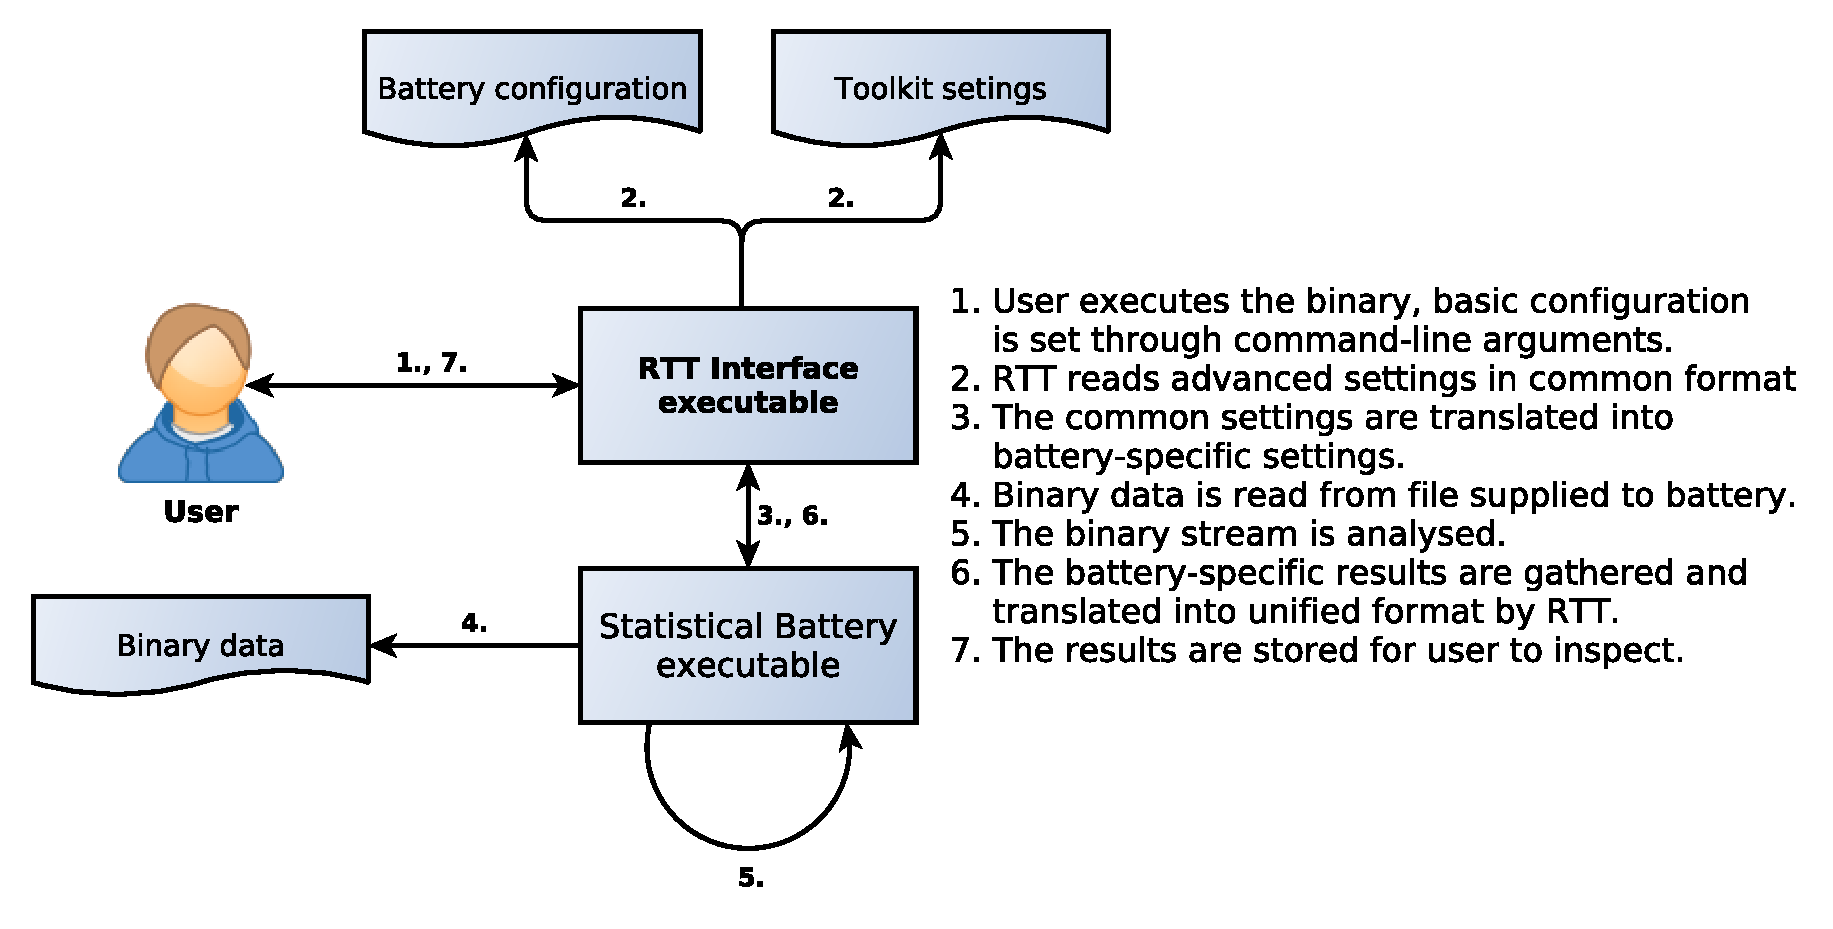
\includegraphics[width=\textwidth]{figures/local-rtt-workflow.pdf} 
\end{nomar}
\end{frame}

\begin{frame}
\frametitle{Randomness Testing Toolkit -- web service}
\begin{nomar}
\centering
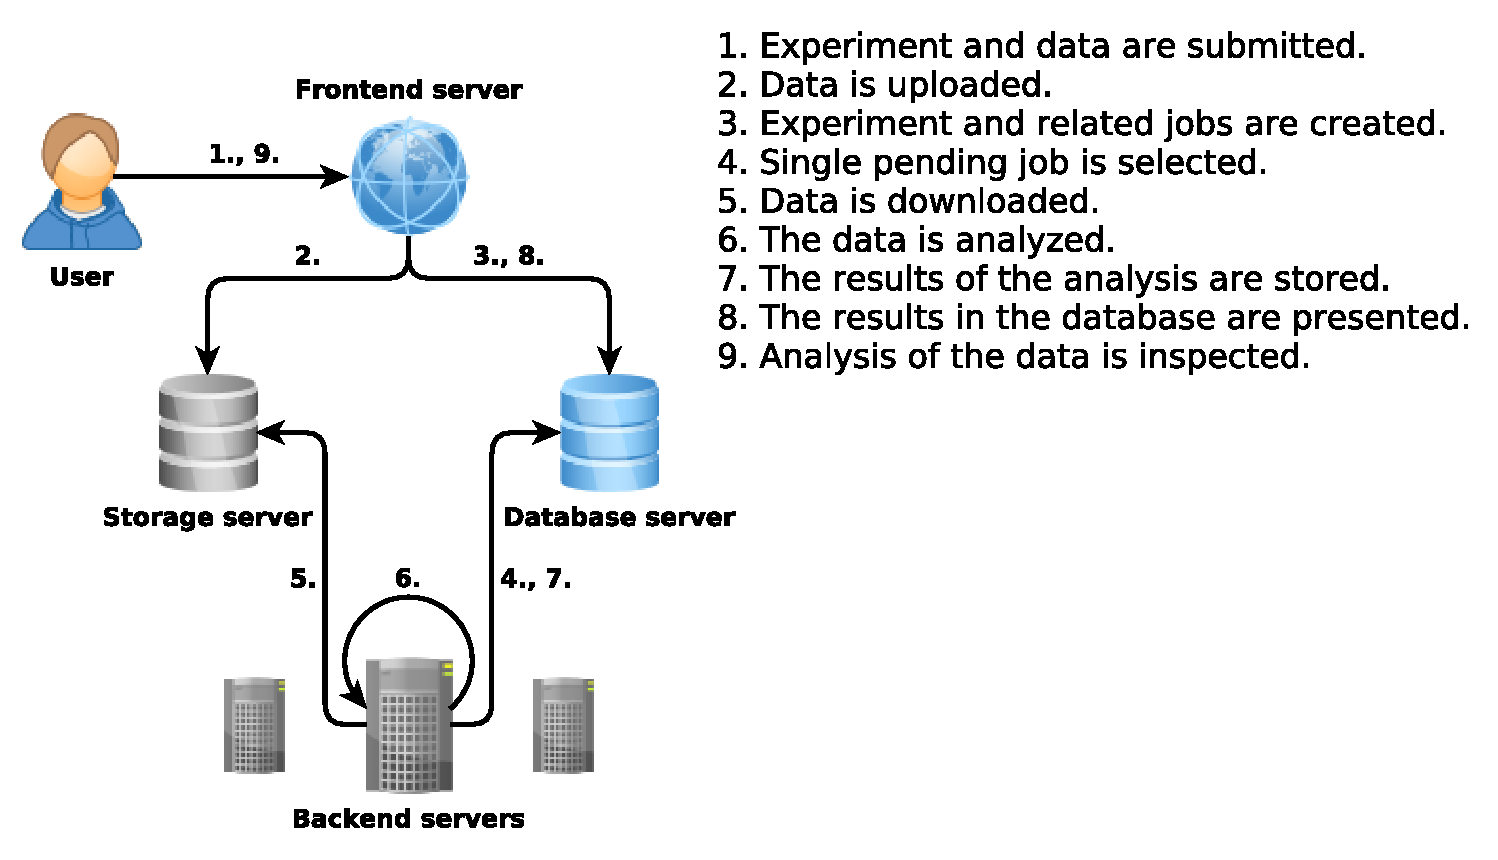
\includegraphics[width=.9\textwidth]{figures/rtt-ecosystem.pdf} 
\end{nomar}
\end{frame}

%%%%%%%%%%%%%%%%%%%%%%%%%%%%%%%%
% Statistical testing overview %
%%%%%%%%%%%%%%%%%%%%%%%%%%%%%%%%
\begin{frame}
\frametitle{Statistical testing of randomness -- 1/2}

\begin{description}
\item[Testing hypothesis -- $H_0$] \hfill \\
During the experiments, we evaluated the hypothesis that the analysed data were produced by a truly random generator. We denote the hypothesis as $H_0$ (null hypothesis).
\item[Statistical battery] \hfill \\
Software with the purpose of detecting biases in data stream; collection of statistical tests.
\item[Statistical test] \hfill \\
Single unit in a statistical battery, checks some property of the data; e.g. count of ones. Output of a test is the probability that the analysed data were produced by TRNG. Each test in a given battery will either fail ($H_0$ rejection) or pass ($H_0$ retainment).
\end{description}

\end{frame}

\begin{frame}
\frametitle{Statistical testing of randomness -- 2/2}

\begin{description}
\item[Significance level -- $\alpha$] \hfill \\
The significance level is set prior to the experiments (usually 0.001) and based on it, the null hypothesis is rejected or retained.
\item[False positive (Type I error)] \hfill \\
The false positive result is observed when $H_0$ holds true but it is rejected -- stream produced by TRNG is evaluated as non random. Probability of Type I error is $\alpha$.
\item[False negative (Type II error)] \hfill \\
The false negative result is observed when $H_0$ is false but it is not rejected -- stream generated by biased generator is evaluated as random.
\end{description}
\end{frame}

%%%%%%%%%%%%%%%%%%%%%%%%%%
% Experiments - baseline %
%%%%%%%%%%%%%%%%%%%%%%%%%%
\begin{frame}
\frametitle{Establishing baseline results}
\begin{itemize}
\item The result of a battery is obtained from the proportion of the failed tests in the battery (e.g. we consider the data biased if more than 2 out of 15 tests fail). However, even data generated by a perfect TRNG may fail some tests (false positives).
\item To identify the maximum count of failed tests (assuming that the $H_0$ holds) we processed 8 TB of data generated by a quantum random generator (control experiment). Further experiments were interpreted based on these results.
\item In order to make the result interpretation more straight-forward, results of certain tests were grouped together. As a consequence, the counts of failed tests are closer to expected (theoretical) numbers and therefore more easy to evaluate.
\end{itemize}
\end{frame}

%%%%%%%%%%%%%%%%%%%%%%%%%%%%%%%%%%
% Experiments - security margins %
%%%%%%%%%%%%%%%%%%%%%%%%%%%%%%%%%%
\begin{frame}
\frametitle{Analysis of well-known algoritms}
\begin{itemize}
\item Analyse outputs of well-known cryptographic algorithms (AES, DES, RC4, etc.).
\item Observe the security margins of the algorithms.
\item Compare the results to other approach in CRoCS.
\end{itemize}

\begin{description}
\item[Analysed algorithms] \hfill \\
\begin{itemize}
\item In total, 72 different data streams were analysed.
\item The data streams were outputs from 16 distinct round-reduced cryptographic algorithms.
\item The algorithms were chosed based on their popularity (AES, DES, RC4, ...) or their success in crypto competitions eSTREAM and SHA3 (Rabbit, Keccak, Gr\o stl, ...).
\end{itemize}
\vspace{.2cm}
\item[Analysis conditions] \hfill \\
\begin{itemize}
\item Each datastream was 8GB long.
\item The conditions of analysis were same as in the previous experiment.
\item The interpretation of the result was based on the results of the baseline experiment.
\end{itemize}
\end{description}

\end{frame}

%%%%%%%%%%%%%%%%%%%%%%%%%%%%%%%%%%
% Experiments - faulty Dieharder %
%%%%%%%%%%%%%%%%%%%%%%%%%%%%%%%%%%
\begin{frame}
\frametitle{Analysis of the results of Dieharder battery}
\begin{itemize}
\item Examine behavior of Dieharder battery during truly random data analysis.
\item Analyse the distribution of the results.
\end{itemize}
\end{frame}

\begin{frame}
\frametitle{Usable testbed analysis -- 2/3}

\begin{table}
\begin{nomar}
\centering

\scalebox{0.75} {
\begin{tabular}{l || r | r | r }
\textbf{Algorithm} & \thead{Biased round \\ RTT} & \thead{Biased round \\ EACirc} & \textbf{Security Margin} \\ \hline \hline
AES        & 3                          & 3  & 7 -- 70\% \\
BLAKE      & 1                          & 1  & 15 -- 93.7\% \\
Grain      & \cellcolor{green!40}6*     & 2  & 7 -- 53.8\% \\
Gr\o stl   & 2                          & 2  & 12 -- 85.7\% \\
HC-128     & --                         & -- & 0 -- 100\% \\
JH         & 6                          & 6  & 36 -- 85.7\% \\
Keccak     & \cellcolor{green!40}3      & 2  & 21 -- 87.5\% \\
MD6        & \cellcolor{green!40}10*    & 8  & 94 -- 90.3\% \\
Rabbit     & \cellcolor{green!40}4*     & 0  & \cellcolor{red!40}0 -- 0\% \\
RC4        & \cellcolor{green!40}0*     & -- & \cellcolor{red!40}0 -- 0\% \\
Salsa20    & 2                          & 2  & 18 -- 90\% \\
SINGLE-DES & \cellcolor{green!40}5      & 4  & 11 -- 68.7\% \\
Skein      & \cellcolor{green!40}4      & 3  & 68 -- 94.4\% \\
SOSEMANUK  & 4                          & 4  & 21 -- 84\% \\
TEA        & \cellcolor{green!40}5      & 4  & 27 -- 84.3\% \\
TRIPLE-DES & \cellcolor{green!40}3      & 2  & 13 -- 81.2\% \\
\end{tabular}
}
\end{nomar}
\end{table}

\end{frame}

%%%%%%%%%%%%%%%%%%%%%%%
% Last official frame %
%%%%%%%%%%%%%%%%%%%%%%%

\begin{frame}

\frametitle{References}
\begin{itemize}
\item \textbf{Randomness Testing Toolkit} \\ \url{https://github.com/crocs-muni/randomness-testing-toolkit}
\item \textbf{EACirc} \\ \url{https://github.com/crocs-muni/eacirc}
\item \textbf{NIST Statistical testing suite} \\ \url{http://csrc.nist.gov/groups/ST/toolkit/rng/documentation_software.html}
\item \textbf{Dieharder} \\ \url{http://www.phy.duke.edu/~rgb/General/dieharder.php}
\item \textbf{TestU01} \\ \url{http://simul.iro.umontreal.ca/testu01/tu01.html}
\end{itemize}

\end{frame}

%%%%%%%%%%%%%%%%%%%%%%%%%%%%%%%%%%
% Additional details and figures %
%%%%%%%%%%%%%%%%%%%%%%%%%%%%%%%%%%

%%%%%%%%%%%%%%%%%%%%%%%%%%%%%%
% Baseline experiment detail %
%%%%%%%%%%%%%%%%%%%%%%%%%%%%%%
\begin{frame}
\frametitle{Baseline experiment -- uncorrected results}
\begin{nomar}
\centering
\includegraphics[width=.85\textwidth]{figures/dieharder-orig.pdf} 
\end{nomar}
\end{frame}

\begin{frame}
\frametitle{Baseline experiment -- corrected results}
\begin{nomar}
\centering
\includegraphics[width=.85\textwidth]{figures/dieharder-corr.pdf} 
\end{nomar}
\end{frame}

\begin{frame}
\frametitle{Baseline experiment -- resulting reference}
\begin{table}
\begin{nomar}
\centering
\begin{tabular}{@{}lrrr@{}}
\toprule
                      & \multicolumn{2}{c}{\textbf{Closeness to expected results}}               &                           \\ \cmidrule(lr){2-3}
\textbf{Battery name} & Uncorrected               & Uncorrected              & \textbf{Allowed failures} \\ \midrule

Dieharder             &    $5.32 \cdot 10^{-17}$  & \gr$0.38$                & 3/27 \\ 
NIST STS              & \gr$2.17 \cdot 10^{-2}$   &    $4.44 \cdot 10^{-7}$  & 2/15 \\ 
TU01 Small Crush      &    $0.71$                 & \gr$0.95$                & 2/10 \\ 
TU01 Crush            &    $3.36 \cdot 10^{-11}$  & \gr$3.31 \cdot 10^{-3}$  & 3/32 \\ 
TU01 Rabbit           & \gr$2.02 \cdot 10^{-5}$   &    $1.45 \cdot 10^{-23}$ & 2/16 \\ 
TU01 Alphabit         &    $2.14 \cdot 10^{-8}$   & \gr$2.8 \cdot 10^{-7}$   & 1/4 \\ 
TU01 Block Alphabit   &    $1.87 \cdot 10^{-68}$  & \gr$5.15 \cdot 10^{-47}$ & 1/4 \\
\bottomrule
\end{tabular}
\end{nomar}
\end{table}
\end{frame}




\begin{frame}
\frametitle{Usable testbed analysis -- 3/3}

\begin{description}
\item[Notable results] \hfill \\
\begin{itemize}
\item \textbf{Grain} -- Tests smarsa\_MatrixRank and scomp\_LinearComp (Crush, Rabbit) will fail in 3, 4, 5 and 6-round configuration.
\item \textbf{MD6} -- Tests smarsa\_MatrixRank and sspectral\_Fourier3 (Crush, Rabbit) will fail in 9 and 10-round configuration.
\item \textbf{Rabbit} -- Tests sstring\_HammingIndep and sstring\_PeriodsInStrings (Crush, Rabbit, Alphabit, Block Alphabit) will fail in \textbf{full} configuration.
\item \textbf{RC4} -- Tests sknuth\_SimpPoker and sknuth\_Gap (Crush) will fail in \textbf{full} configuration.
\end{itemize}
\end{description}

\end{frame}

\begin{frame}
\frametitle{Analysis of Dieharder -- 1/2}

\begin{description}
\item[Analysed data] \hfill \\
\begin{itemize}
\item 8TB of quantum random data processed continuously by the tests - single application of a test to a data stream will yield single first-level p-value
\item Uniformity of the first level p-values was analysed.
\item The p-values should be uniformly distributed on the interval $<0,1>$.
\item Total of 110 sets of p-values (single set per raw, uncorrected test) was inspected.
\item Each set had a different size -- usually between 1 to 2 millions of p-values per set.
\end{itemize}
\vspace{.2cm}
\item[Experiment results] \hfill \\
\begin{itemize}
\item Out of 110 p-value sets, 39 sets were not uniformly distributed
\item Chi-Square ($\chi^2$) statistic used for uniformity testing. When the p-value of the statistic was less than 0.001, the inspected set was considered non-uniform.
\item Flawed non-uniform distributions can have impact on Dieharder results.
\end{itemize}
\end{description}

\end{frame}

\begin{frame}
\frametitle{Analysis of Dieharder -- 2/2}

\begin{figure}
\begin{nomar}
\centering
\includegraphics[width=.45\paperwidth]{figures/011.png} 
\includegraphics[width=.45\paperwidth]{figures/100.png}
\end{nomar}
\end{figure}

\end{frame}

\end{document}
